\documentclass[11pt]{report}
\usepackage[french]{babel}
\usepackage[utf8]{inputenc}
\usepackage[T1]{fontenc}
\usepackage[top = 1.5cm, bottom = 1.5cm, left = 1cm, right = 1cm]{geometry}
\usepackage{fancyvrb}
\usepackage{mathalfa}
\usepackage{amsfonts}
\usepackage[table]{xcolor}
\usepackage{amsmath}
\usepackage{graphicx}
\usepackage{listings}
\usepackage{color}
\usepackage{times}
\usepackage{cprotect}
\usepackage{parskip}

\definecolor{black}{rgb}{0, 0, 0}
\definecolor{darkPink}{rgb}{1.0, 0, 1.0}
\definecolor{darkGreen}{rgb}{0, 0.4, 0}

\lstdefinelanguage{myPython}
{
	morecomment=[l]{\%},
	%morecomment=[s]{"""}{"""}
	%morestring=[b]"
}

\lstset
{
	language = {myPython},
	backgroundcolor=\color{cyan!10},
	basicstyle=\small\tt,
	breakatwhitespace=false,
	breaklines=true,
	commentstyle=\color{darkGreen},        
	keepspaces=true,  
	keywords = [1]{for, while, if, end, function},
	keywordstyle = [1]\color{blue},
	keywords = [2]{load, size, extractHOGFeatures, fitcsvm, fitensemble, rgb2gray, mean2, std2, im2double, imresize, predict, abs, char, strcat, fprintf, fopen, fclose},
	keywordstyle = [2]\color{darkPink},
	keywords = [3]{normalize},
	keywordstyle = [3]\color{red},   
	numbers=left,                   
	numbersep=1em,                  
	numberstyle=\tiny\color{black},       
	showspaces=false,                
	showstringspaces=false,          
	showtabs=false,           
	stepnumber=1,              
	stringstyle = \color{grey!10},    
	tabsize = 4
}

\renewcommand{\thesection}{\arabic{section}}
\pagestyle{empty}

\begin{document}

\noindent
\textbf{Hachem BENYAHIA \hfill 22 mai 2016}

\begin{center}
\section*{Rapport SY32 - Partie 2 ~\\ Construction d'un détecteur de visages}
\rule{\textwidth}{2pt}
\end{center}

\subsection*{Ensemble d'entraînement}

Pour permettre au détecteur de détecter des visages, il faut d'abord savoir ce qu'est un visage. Il faut donc apprendre à un ou plusieurs classifieurs à reconnaître un visage à partir d'un grand nombre nombre d'observations et leur classes associées. En l'occurrence les deux classes possibles sont \textbf{visage} ($1$ dans l'implémentation) et \textbf{non visage} ($0$ dans l'implémentation).

Les données utilisées pour les visages sont celles du TD2. Plutôt que la version imagée, j'ai pris directement la version matrice qui est également disponible sur le moodle de l'UV. En effet, elle raccourcit (et simplifie) énormément le traitement et l'exécution des images. Dans la suite, j'ai par ailleurs essayé de sauvegarder les variables le plus possible dans des fichiers pour rendre le code plus modulaire et rapide à l'exécution.

On dispose donc initialement des fichiers \verb|neg.mat| et \verb|pos.mat| (que j'ai renommés en \verb|negatives.mat| et \verb|positives.mat|) qui contiennent respectivement les variables \verb|neg| (un tableau de $17256$ images \textbf{non visage}) et \verb|pos| (un tableau de $4000$ images \textbf{visage}). Les images sont toutes en noir et blanc et en $24 \times 24$ pixels. Ces $21256$ images constituent donc l'ensemble d'entraînement des classifieurs qu'on utilisera par la suite pour déterminer si une image est un visage ou pas. Par la suite, nous appellerons les images représentant un visage \textbf{images positives} et les autres \textbf{images négatives}.

\begin{figure}[h]
\centering
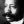
\includegraphics{image/pos.png}
\cprotect\caption{Une image positive (visage)}
\end{figure}

\begin{figure}[h]
\centering
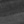
\includegraphics{image/neg.png}
\cprotect\caption{Une image négative (non visage)}
\end{figure}

\subsection*{Extraction des caractéristiques}

Les images en elles-mêmes ne sont pas représentatives de grand-chose, en tant qu'ensemble de pixels. Elle ne sont pas pertinentes pour l'apprentissage des classifieurs. C'est pourquoi on utilisera les \textbf{caractéristiques} de l'image plutôt que l'image en tant que telle. J'ai entraîné tous les classifieurs sur la base des vecteurs de \textbf{gradient orienté} (HOG, \textit{Histogram of Oriented Gradient}). Pour que les caractéristiques obtenues soient cohérentes d'une image à l'autre de la même classe, j'ai d'abord mis les images en noir et blanc (les images de l'ensemble d'apprentissage étaient déjà en noir et blanc, mais cette opération vaudra aussi pour les images de test comme nous le verrons après). Ensuite il faut normaliser les images pour éviter que leurs valeurs soient trop dispersées (écarts dûs à l'éclairage notamment). La normalisation d'une image au sens où je l'entends est de faire suivre à ses pixels une \textbf{loi normale centrée réduite}, c'est-à-dire $\forall i,j$ indices du pixel $p$ de l'image : 

$$
p'(i, j) = \frac{p(i, j) - M}{\sigma}
$$

où $p'$ est la nouvelle valeur du pixel, $M$ est la moyenne des pixels de l'image, et $\sigma$ leur écart-type.

Une fois que l'image est normalisée, on peut extraire son vecteur de gradient. Remarquons que comme toutes les images sont de la même taille (ce qui est fait exprès), leurs vecteurs de caractéristiques font tous la même taille. En l'occurrence, des vecteurs de taille $1 \times 144$ pour des images $24 \times 24$.

\subsection*{Constitution des observations et des classes}

Pour pouvoir appeler les fonctions de \textbf{Matlab} qui construisent des \textbf{classifieurs} (SVM, \textit{Support Vector Machine}), il faut leur fournir des observations et le vecteur de classes (prédictions théoriques) associé. Plus formellement, si $c_{i}$ est le vecteur de caractéristiques $1 \times 144$ (décrit précédemment) de l'image $i$, alors la matrice des observations $X$ sera la concaténation sur $i$ de tous ces vecteurs :


$$
X = 
\left[
\begin{array}{c}
c_{1} \\
c_{2} \\
\vdots \\
c_{n - 1} \\
c_{n} \\
\end{array}
\right]
$$

Le vecteur des classes $Y$ vaudra $1$ là où les caractéristiques proviennent d'une image de visage, et $-1$ là où ils proviennent d'une image de non-visage. Plus formellement, si $n_{1}$ est le nombre de visages de l'ensemble d'entraînement et $n_{2}$ le nombre de non-visages , alors il contiendra $n_{1} ~~ 1$ et $n_{2} ~~ -1$. En supposant donc que les caractéristiques dans $X$ soient ordonnées avec les $n_{1}$ vecteurs horizontaux en premiers et ensuite les $n_{2}$ autres vecteurs, on aurait un $Y$ avec cette structure : 

$$
Y = 
\left[
\begin{array}{c}
1 \\
1 \\
\vdots \\
1 \\
1 \\
-1 \\
-1 \\
\vdots \\
-1 \\
-1 \\
\end{array}
\right]
$$

\subsection*{Apprentissage des classifieurs}

Une fois que ces structures sont mises en place, il suffit d'appeler les fonctions correspondantes de \textbf{Matlab} pour apprendre aux classifieurs à reconnaitre les visages. Le code ci-dessous lit les images, les normalise, extrait leurs caractéristiques, constitue la matrice $X$ et le vecteur $Y$ et apprend ces modèles à différents classifieurs :

\begin{lstlisting}
load('positives.mat');
load('negatives.mat');

X = [];
Y = [];

positives = {};
negatives = {};

for i = 1 : size(pos, 3)
    positives{i} = pos(:, :, i);
    positives{i} = normalize(positives{i});
    X = [X ; extractHOGFeatures(positives{i})];
    Y = [Y ; 1];
end

for i = 1 : size(neg, 3)
    negatives{i} = neg(:, :, i);
    negatives{i} = normalize(negatives{i});
    X = [X ; extractHOGFeatures(negatives{i})];
    Y = [Y ; -1];
end

svm1 = fitcsvm(X, Y) 
svm2 = fitensemble(X, Y, 'AdaboostM1', 100, 'Tree')
svm3 = fitensemble(X, Y, 'RUSBoost', 500, 'Tree')
svm4 = fitensemble(X, Y, 'Subspace', 2000, 'Discriminant');
\end{lstlisting}

où \verb|normalize| est la fonction de normalisation suivante : 

\begin{lstlisting}
function [M] = normalize(M)
    if(size(M, 3) == 3)
        M = rgb2gray(M);
    end
    M = im2double(M);
    mean = mean2(M);
    std = std2(M);
    M = (M - mean) / std;
end
\end{lstlisting}

Finalement, on obtient $4$ classifieurs listés dans l'ordre de puissance plus ou moins capables de distinguer une image positive d'une image négative.

\newpage
\subsection*{Fenêtre glissante et détection}

L'algorithme de détection de visage repose sur un principe simple : il suffit de découper une image en morceaux et d'identifier si celle-ci est une image positive ou négative. En pratique, chaque image est parcourue de la manière suivante par une \textbf{fenêtre} : 

\begin{figure}[h]
\centering
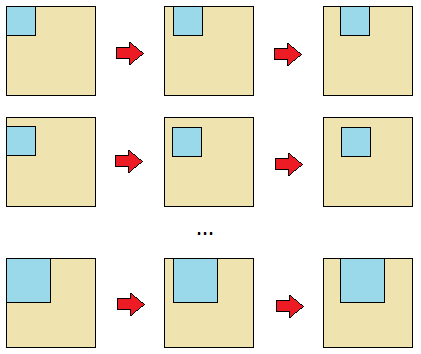
\includegraphics{image/fenetre-glissante.png}
\cprotect\caption{Algorithme de fenêtre glissante : la fenêtre (en bleu) parcourt l'image (en beige)}
\end{figure}

On démarre avec une taille de fenêtre de $24 \times 24$ (j'ai fait le choix de la fenêtre carrée car cela simplifie grandement l'implémentation sans nécessairement changer grand-chose au résultat ; de plus, les classifieurs ont été entraînés sur des images carrées, il vaut donc mieux leur fournir des images de test carrées pour maximiser leurs chances de faire une bonne prédiction). 

La fenêtre est idéalement déplacée d'un seul pixel à chaque itération, mais en pratique cela prendrait énormément de temps, donc le déplacement se fait de plusieurs pixels à chaque fois. Après avoir parcouru toute l'image, la fenêtre augmente de taille et continue son parcours, jusqu'à identifier un visage (détection), auquel cas l'algorithme s'arrête.

~\\
Voici le code de l'algorithme décrit ci-dessus :

\begin{lstlisting}
load('svm1.mat'); % les svms crees enregistres dans des fichiers
load('svm2.mat');
load('svm3.mat');
load('svm4.mat');
load('tests.mat'); % les images de tests
load('names.mat'); % les noms des images de tests

jump = 15; % le saut fait a chaque deplacement de la fenetre
jumpWindow = 20; % l'augmentation de la taille de la fenetre a chaque iteration

for k = 1 : size(tests, 2)
    M = tests{k}
    data = [];
    scores = [];
    windowSize = 24; % taille initiale de la fenetre
    maxSize = min(size(M, 1), size(M, 2)); % taille maximum de la fenetre
    
    while (windowSize < maxSize)
        for i = 1 : jump : (size(M, 1) - windowSize)
            for j = 1 : jump : (size(M, 2) - windowSize)
                window = imresize(M(i : (i + windowSize), j : (j + windowSize)), [24 24]); 
                window = normalize(window); 								
                X = extractHOGFeatures(window);

                [label, score] = predict(svm1, X);
%                 if label == 1
%                     [label, score] = predict(svm2, X);
%                     if label == 1
%                         [label, score] = predict(svm3, X);
%                         if label == 1
%                             [label, score] = predict(svm4, X);
%                             if label == 1
%                            		%return;
%                             end
%                         end
%                     end
%                 end

                data = [data ; i j windowSize label]; % les donnees associees a la fenetre
                scores = [scores ; abs(score(1))]; % le score associe a la fenetre
            end
        end

        windowSize = windowSize + jumpWindow; % augmentation de la fenetre
    end
    
    % enregistrement des donnees dans les fichiers
    name = char(strcat(names(k), '.txt')); % le nom est au format '0001.jpg.txt'
    fid = fopen(name,'wt');
    for m = 1 : size(data, 1)
        fprintf(fid, '%d\t', data(m, :));
        fprintf(fid, '%.2f\t', scores(m));
        fprintf(fid, '\n');
    end
    fclose(fid);
end
\end{lstlisting}

A chaque fenêtre, on redimensionne l'image considérée à la taille $24 \times 24$ (car les classifieurs ont été entrainés sur cette taille) et on la normalise. On extrait ensuite son vecteur de caractéristiques et on utilise les classifieurs pour obtenir une prédiction de la classe de ce vecteur. 

J'ai mis en commentaire la plupart des classifieurs pour la même raison que j'ai mis des sauts \verb|jump| et \verb|jumpWindow| très supérieurs à $1$ pixel : car le temps de calcul est beaucoup trop élevé. En fait, l'exécution de cette algorithme sur les $447$ images de test prend déjà plus d'une heure. Si on mettait les saut à 1 pixel, il faudrait compter plusieurs heures. Et encore plus en utilisant la cascade de classifieurs. 

Les variables que j'ai chargées sont des variables que j'ai enregistrées \textit{une bonne fois pour toutes} avec la fonction \verb|save()| de \textbf{Matlab}. En effet, comme je l'ai dit en introduction de ce rapport, l'exécution est infiniment plus rapide en chargeant simplement les variables qu'en rééxécutant à chaque fois le code qui les génère.

\newpage
\subsection*{Organisation du code}

Le repertoire \verb|code| contient un certains nombre de fichiers \verb|.m| et \verb|.mat|. Les fichiers\verb|.m| sont des fichiers de code et les fichiers \verb|.mat| sont des fichiers de variables (à utiliser dans un code via la méthode \verb|load()|). Voici la liste du contenu de \verb|code| :

~\\
Les fichiers de code :

\paragraph*{\protect\Verb+main.m+}

L'algorithme de la fenêtre glissante. C'est le script principal.

\paragraph*{\protect\Verb+svms.m+}

Le code pour générer les $4$ classifieurs.

\paragraph*{\protect\Verb+normalize.m+}

La fonction de normalisation d'une image.

\paragraph*{\protect\Verb+tests.m+}

Le fichier qui génère les images de tests et leurs noms.

~\\
Les fichiers de variable :

\paragraph*{\protect\Verb+positives.mat+}

Les images d'entraînement positives.

\paragraph*{\protect\Verb+negatives.mat+}

Les images d'entraînement négatives.

~\\
Pour exécuter le code, il faut d'abord générer les variables que \verb|main.m| utilise. Il faut donc lancer dans l'ordre : \verb|tests.m|, \verb|svms.m| puis \verb|main.m|.

\subsection*{Fichiers de log}

Les fichiers portent le nom de l'image concaténé à \verb|.txt|. Par exemple, l'image de test \verb|0001.jpg| correspond au fichier \verb|0001.jpg.txt|. 

Chaque ligne contient $5$ colonnes : la coordonnée $i$ (la ligne) du coin supérieur gauche de la fenêtre, la coordonnée $j$ (la colonne) du coin supérieur gauche de la fenêtre, la taille (la hauteur est égale à la largeur) de la fenêtre, la classe prédite par le classifieur, et le score renvoyé par la fonction \verb|predict()| (la probabilité que la prédiction soit correcte).

Les fichiers ont été généré avec le code ci-dessous :

\begin{lstlisting}
load('svm1.mat');
load('svm2.mat');
load('svm3.mat');
load('svm4.mat');
load('names.mat');
load('tests.mat');

jump = 15;
jumpWindow = 20;

for k = 1 : size(tests, 2)
    M = tests{k}
    data = [];
    scores = [];
    windowSize = 24;
    maxSize = min(size(M, 1), size(M, 2));
    while (windowSize < maxSize)
        for i = 1 : jump : (size(M, 1) - windowSize)
            for j = 1 : jump : (size(M, 2) - windowSize)
                window = imresize(M(i : (i + windowSize), j : (j + windowSize)), [24 24]);
                window = normalize(window);
                X = extractHOGFeatures(window);

                [label, score] = predict(svm1, X);

                data = [data ; i j windowSize label]; 
                scores = [scores ; abs(score(1))];
            end
        end

        windowSize = windowSize + jumpWindow;
    end
    
    name = char(strcat(names(k), '.txt'));
    fid = fopen(name,'wt');
    for m = 1 : size(data, 1)
        fprintf(fid, '%d\t', data(m, :));
        fprintf(fid, '%.2f\t', scores(m));
        fprintf(fid, '\n');
    end
    fclose(fid);
end
\end{lstlisting}

\end{document}